% vim: set textwidth=78 autoindent:

\subsection{Interpolation Plugin}

% when the revision of a section has been finalized, 
% comment out the following line:
%\updatedisclaimer

The Interplation plugin allows to interpolate a TIN or IDW raster layer from a vector 
point layer loaded in the QGIS canvas. It is very simple to handle and provides 
functionalities as shown in Figure \ref{fig:interpolation_dialog}.

\begin{itemize}
\item \textbf{Input vector layer}: Select vector point layer loaded in the QGIS canvas.
\item \textbf{Interpolation attribute}: Select attribute column used for interpolation or 
enable \checkbox{Use Z-Coordinate} checkbox.
\item \textbf{Interpolation Method}: Select interpolation method \selectstring{Triangulated Irregular 
Network (TIN)}{\ldots} or \selectstring{Inverse Distance Weighted (IDW)}{\ldots}.
\item \textbf{Number of columns/rows}: define number colums and.rows for the output raster file
\item \textbf{Output file}: Define a name for the output raster file
\end{itemize}

\begin{figure}[ht]
   \begin{center}
   \caption{Interpolation Plugin \nixcaption}\label{fig:interpolation_dialog}\smallskip
   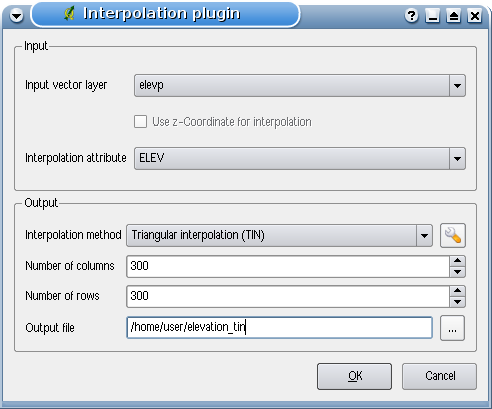
\includegraphics[clip=true, width=9cm]{interpolate_dialog}
\end{center}  
\end{figure}

\begin{enumerate}
  \item Start QGIS and load the \filename{elevp.csv} CSV table with elevation points in the QGIS 
  canvas using the delimited text plugin as described in Section \ref{label_dltext}. 
  \item Load the Interpolation plugin in the Plugin Manager (see Section 
  \ref{sec:load_core_plugin}) and click on the \toolbtntwo{interpolation}{Interpolation} 
  icon which appears in the QGIS toolbar menu. The Interpolation plugin dialog appears as shown in Figure \ref{fig:interpolation_dialog}.
  \item Select \selectstring{elevp}{\ldots} as input vector and column \filename{ELEV} for 
  interpolation.
  \item Select \selectstring{Triangular interpolation}{\ldots} as interpolation method, define 
  3663 cols and 1964 rows (this is equivalent to a 1000 meter pixel resolution) as raster 
  output filename \filename{elevation\_tin}.
  \item Click \button{Ok}.
  \item Double click \filename{elevation\_tin} in the map legend to open the Raster Layer Properties 
  dialog and select \selectstring{Pseudocolor}{\ldots} as Color Map in the \tab{Symbology} tab. Or you 
  can define a new color table as described in Section \ref{label_rasterprop}.
\end{enumerate}

In Figure \ref{fig:interpolation_idw} you see the IDW interpolation result with a 366 cols x 196 rows (10 km) 
resolution for the \filename{elevp.csv} data visualized using the Pseudocolor color table. The processing 
takes a couple of minutes, although the data only cover the northern part of Alaska.

\begin{figure}[ht]
   \begin{center}
   \caption{Interpolation of elevp data using IDW method \nixcaption}\label{fig:interpolation_idw}\smallskip
   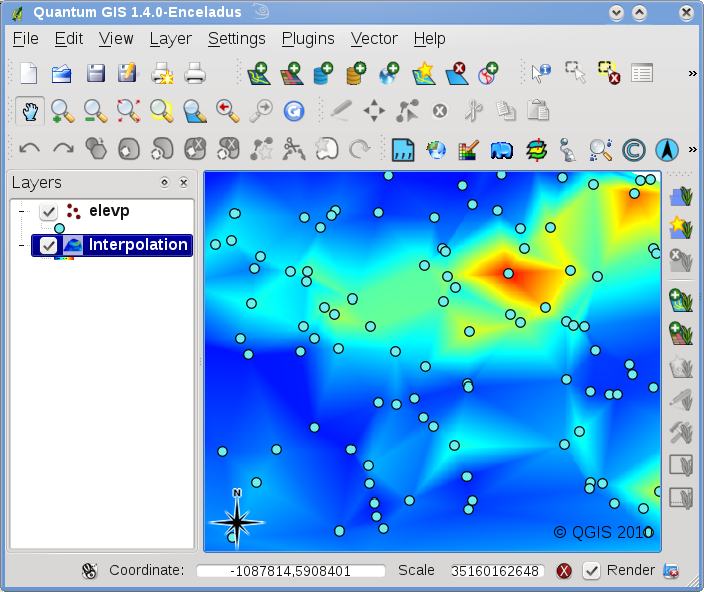
\includegraphics[clip=true, width=\textwidth]{interpolate_idw}
\end{center}  
\end{figure}

\newpage



